\documentclass[tikz,border=6pt]{standalone}
\usepackage[T1]{fontenc}
\usepackage{helvet}
\renewcommand{\familydefault}{\sfdefault}
\usetikzlibrary{arrows.meta}
\tikzset{
  box/.style={draw,thick,minimum width=3.6cm,minimum height=1.6cm,align=center,font=\small},
  arr/.style={-{Stealth[length=2.5mm]},thick},
  lab/.style={font=\scriptsize,align=center}
}
\begin{document}
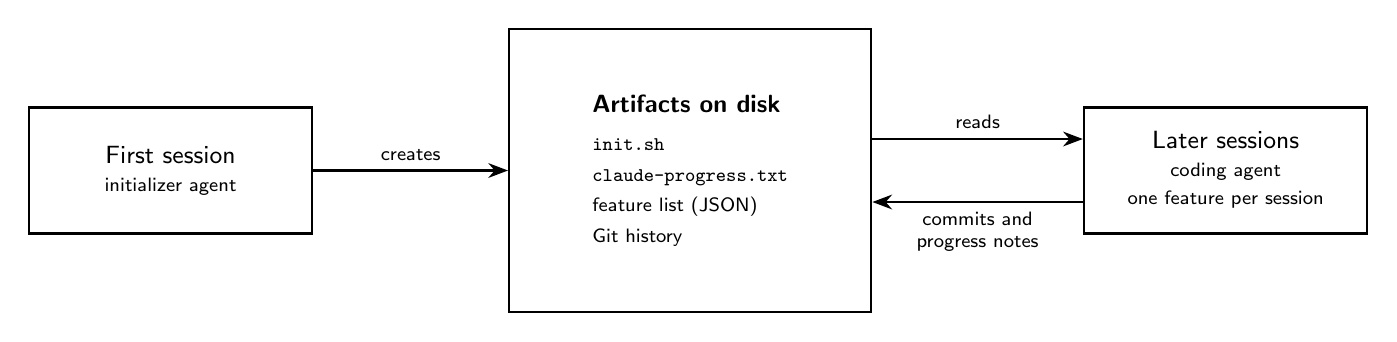
\begin{tikzpicture}
  \node[box] (init) at (0,0) {First session\\[-1pt]{\scriptsize initializer agent}};

  \node[draw,thick,minimum width=4.6cm,minimum height=3.6cm,align=left,font=\small] (art) at (6.6,0)
    {\textbf{Artifacts on disk}\\[3pt]
     {\scriptsize \texttt{init.sh}}\\
     {\scriptsize \texttt{claude-progress.txt}}\\
     {\scriptsize feature list (JSON)}\\
     {\scriptsize Git history}};

  \node[box] (code) at (13.4,0) {\begin{tabular}{c}
      Later sessions\\[-1pt]
      {\scriptsize coding agent}\\[-1pt]
      {\scriptsize one feature per session}
    \end{tabular}};

  \draw[arr] (init) -- node[lab,above] {creates} (art);
  \draw[arr] ([yshift=0.4cm]art.east) -- node[lab,above] {reads} ([yshift=0.4cm]code.west);
  \draw[arr] ([yshift=-0.4cm]code.west) -- node[lab,below] {commits and\\progress notes} ([yshift=-0.4cm]art.east);
\end{tikzpicture}
\end{document}
